\section{基于U-Net和GAN网络的深度学习方法}
\label{sec:gan}


\subsection{大规模可见水印检测和去除数据集}
由于可见水印的多样性,设计鲁棒的可见水印检测和去除方法仍然是一项具有挑战性的任务。具体而言,可见水印可能由文字、符号、图形等组成,导致从未知和多样化的水印模式中提取有区分性的特征较为困难。此外,各种类型的水印图像在嵌入过程中其形状、位置、透明度和大小的变化使得在实际情况下估计水印嵌入区域变得更加困难。现有的可见水印检测和去除工作需要通过从图像中提取手工设计的特征,高度依赖先验知识,抑或是假设水印图像具有相同的水印模式。这种强先验依赖或约束都不适用于在水印可能是未知的、不同图像中的水印更可能是不同的真实场景。而深度卷积网络基于大量图像数据学习特征表示的强大性能,但使得其对未知和多样化水印模式的检测和去除成为可能。

\begin{figure}[!htbp]
	\centering
	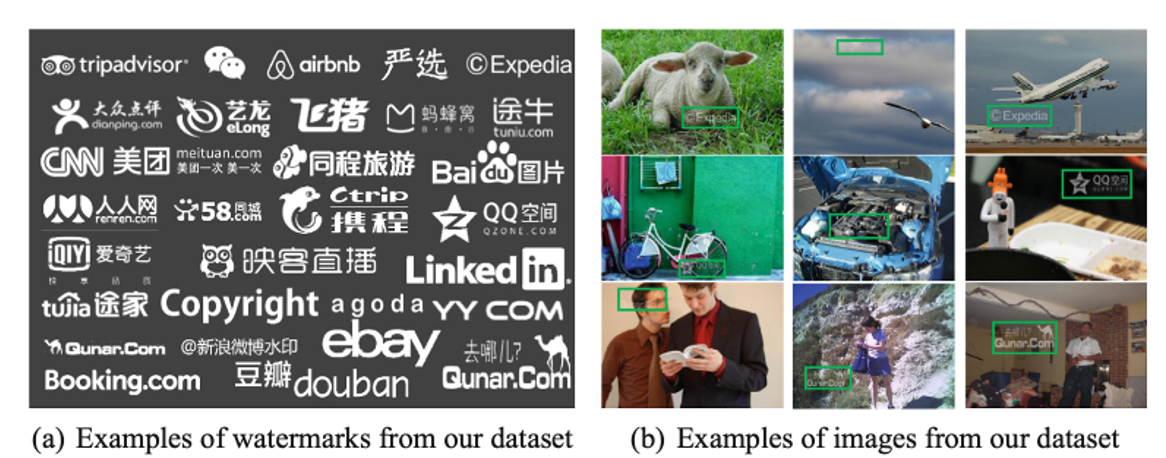
\includegraphics[width=\columnwidth]{17.png}
	\caption{数据集示例图}
	\label{fig:17}
\end{figure}

在水印检测和去除方面,既没有基于深度学习的方法,也缺乏大规模的水印数据集。为了填补这一空白,Cheng 等~\cite{cheng2018large}制作了一个包含60000张由80个水印制成的带水印图像数据集,每个水印有750张图像。具体而言,训练和测试集中使用的原始图像是采用有放回抽样分别从PASCAL VOC2012数据集的训练/验证集和测试集中随机选择的。而80个水印类别采集自知名的电子商务品牌、网站、组织、个人等,涵盖了大量的模式(如包括英文和中文)。此外,不同图像中每个水印的大小、位置和透明度在嵌入时都是随机设置的。该数据集与传统的小规模水印数据集之间的另一个重要区别在于,训练集中的水印不用于构建测试集中的图像。具体而言,在现有的水印数据集中,训练集和测试集中的水印完全相同。这将导致在这种数据集上训练的水印检测器无法很好地检测图像中的未知水印。

\begin{figure*}[!htbp]
	\centering
	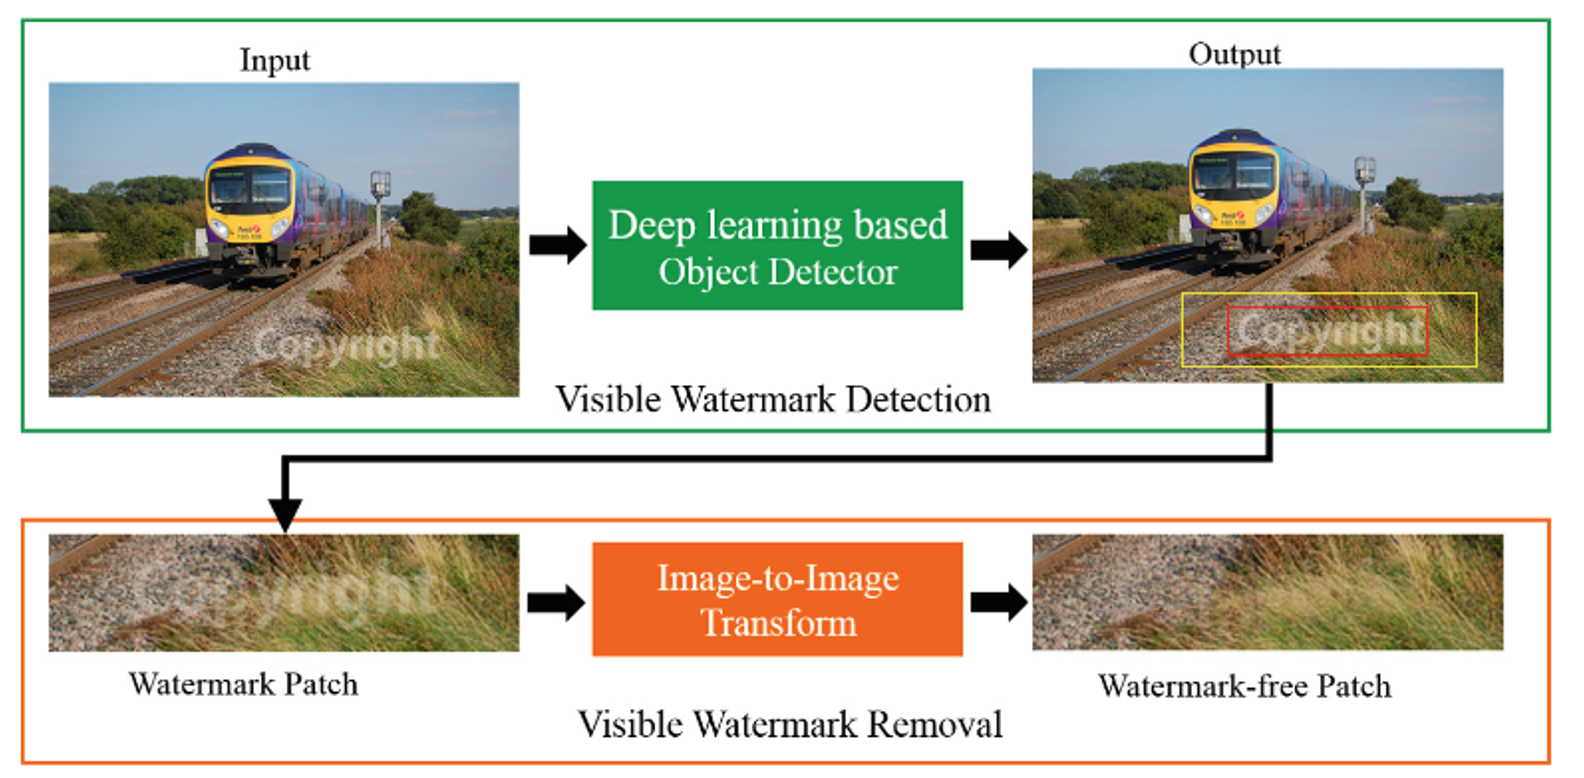
\includegraphics[width=\linewidth]{18.png}
	\caption{可见水印处理框架示意图}
	\label{fig:18}
\end{figure*}

其设计的可见水印处理框架由水印检测和去除两个部分组成。具体而言,采用当前最先进的目标检测器框架作为水印检测网络,如Faster RCNN、YOLO、RetinaNet,并对其进行进一步微调以适应在图像中检测和定位可见水印的任务。一旦图像中的水印被准确检测出来,检测结果可以用于进一步的水印去除。

在去除过程中,将水印去除转化为图像到图像的转换问题,有效地将带水印的像素转换为原始的未标记像素。这一部分包括水印去除网络和损失网络。每个带水印的图像块x被输入到水印去除网络中,以获取估计的无水印图像块˜y。水印去除网络为U-Net架构,其在结构上具有镜像对称性,并且在相应的块之间具有跳跃连接。通过这种方式,使得输入附近的浅层特征与高层特征结合在一起,以便保留输入图像的位置和纹理等低层特征。

\begin{figure}[!htbp]
	\centering
	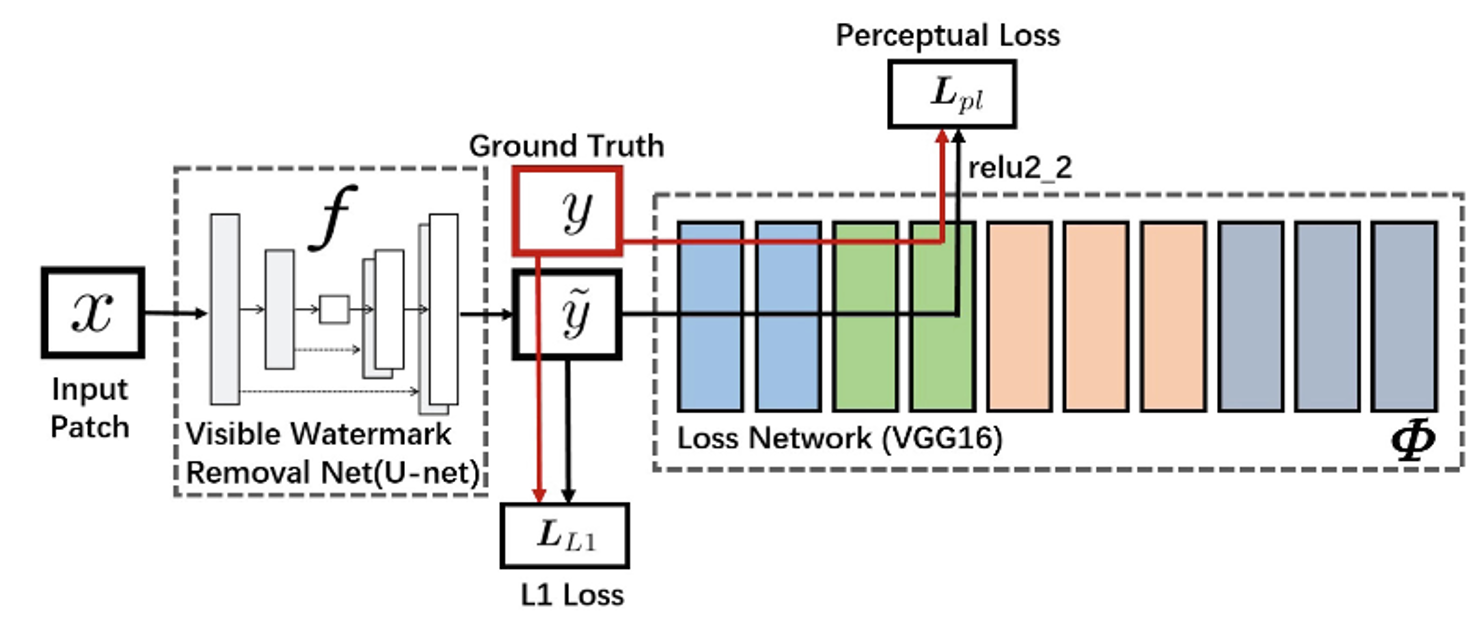
\includegraphics[width=\columnwidth]{19.png}
	\caption{可见水印去除网络架构图}
	\label{fig:19}
\end{figure}

然后,基于真值和估计的图像块计算L1损失和感知损失。与将整个图像进行像素级别的转换不同,该工作侧重于将检测到的区域内的像素恢复到未标记的状态,而水印图像中未标记区域内的像素将保持不变。由于L1损失是基于整个图像逐像素计算的,当每个像素有微小变化且图像在视觉上几乎没有差异时,L1损失会很大。而感知损失被证明在捕捉源图像的语义信息方面是有效的,它依赖于来自卷积层的高级特征,因此,使用感知损失可以得到更加真实的输出结果。

\begin{equation}
\boldsymbol{L}_{\text {whole }}=\boldsymbol{L}_{L 1}+\alpha \boldsymbol{L}_{p l}^{\Phi, \text { relu2 } \_2}
\end{equation}

\begin{equation}
\boldsymbol{L}_{L 1}(x, y)=\|f(x)-y\|_1
\end{equation}

\begin{equation}
\boldsymbol{L}_{p l}^{\Phi, j}(\tilde{y}, y)=\frac{1}{C_i H_i W_i}\left\|\Phi_j(\tilde{y})-\Phi_j(y)\right\|_2^2
\end{equation}

\subsection{更真实的可见水印去除网络}

在传统的可见水印去除方法中,存在两个主要问题。首先,在执行水印去除之前,需要手动标记水印图像中的水印区域和非水印区域。其次,为了有效地去除水印,需要多个具有相同水印的水印图像进行水印去除。Cheng等首次将卷积神经网络引入水印去除任务,有效解决上述两个问题。然而,由于直接训练具有像素级损失的生成器来建模像素映射关系是较为困难的,再加上且他们采用的网络结构简单、损失函数效率低下,他们模型得到的结果并不理想。通过其方法恢复的无水印图像通常仍然包含一些残留的水印痕迹,使得恢复的图像在人类视觉感知上不具备真实感。

\begin{figure}[!htbp]
	\centering
	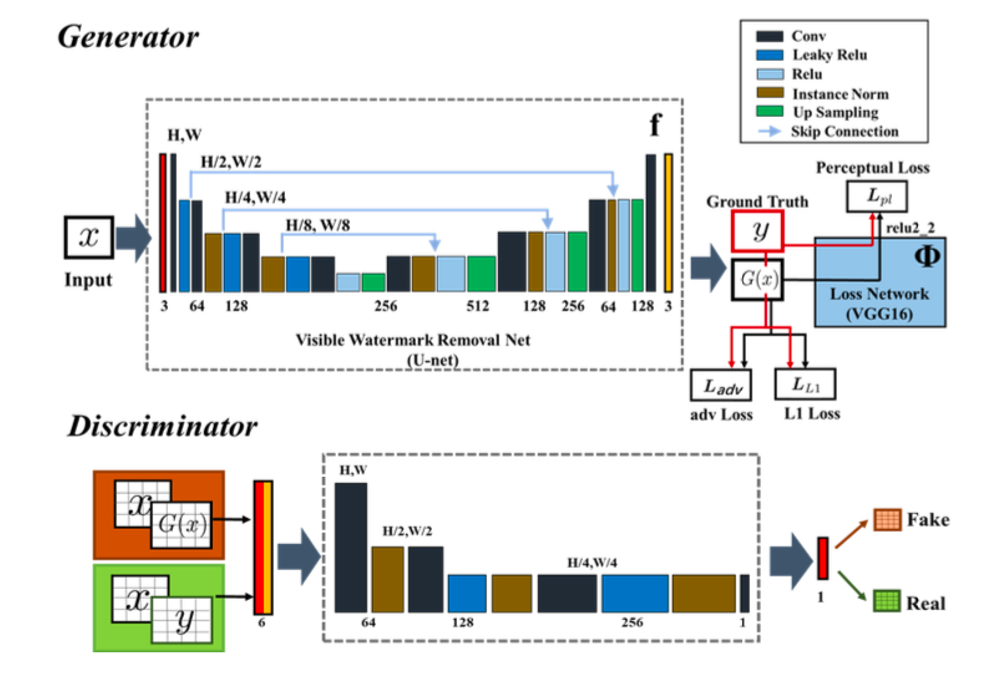
\includegraphics[width=\columnwidth]{20.png}
	\caption{基于条件生成对抗网络的可见水印去除网络架构图}
	\label{fig:20}
\end{figure}


为了使水印去除的结果更具照片般的真实感和可信度(例如,恢复没有任何残留水印的水印区域并使其更具照片般的真实感),Li等~\cite{li2019towards}基于条件生成对抗网络(conditional generative adversarial networks, cGANs)设计了一个照片般真实水印去除的框架。该网络由一个生成器和一个判别器组成,基于U-Net架构的生成器以嵌入了水印的图像作为输入,生成一个逼真的无水印图像。判别器是一个基于图像块的分类器,与常见的GAN判别器将输入映射为表示输入样本“真实”概率的标量不同,它将水印图像和去水印图像的组合映射为特征图,用以表示输入的图像块的“假”或“真”类别概率。由于特征图中的点可以追溯到原始图像中的特定感受野,因此输出矩阵中的每个值表示原始图像中的块是否“真实”的概率。规定输入图像是“真实”的概率为所有图像块为“真实”的概率的平均值。这样做是因为水印图像与原始无水印图像之间的差异仅存在于图像的某些部分。由于水印区域相对于整个图像来说比较小,基于图像块的判别器能够识别两个输入图像的最不同的区域并更加关注最小化这些区域的重建误差。

除此以外,为了使生成器恢复的图像尽可能接近真实的无水印图像,在Cheng等损失函数的基础上引入了新的目标函数,即最终目标函数由 L1 损失、感知损失和基于图像块的对抗损失函数的组成,用于约束生成器的训练。同时,使用一个经过对抗训练的判别器 D 来区分“假”图像和真实图像。

\begin{equation}
\boldsymbol{G}^*=\arg \min _G \max _D \underbrace{\boldsymbol{L}_{\text {adv }}(G, D)}_{\text {adversarial loss }}+\underbrace{\alpha \boldsymbol{L}_{l_1}(G)+\beta \boldsymbol{L}_{p e r}(G)}_{\text {content loss }} .
\end{equation}

\begin{equation}
\boldsymbol{L}_{a d v}(G, D)=\mathbb{E}_{x, y}[\log D(x, y)]+\mathbb{E}_x[\log (1-D(x, G(x)))]
\end{equation}

\begin{figure}[!htbp]
	\centering
	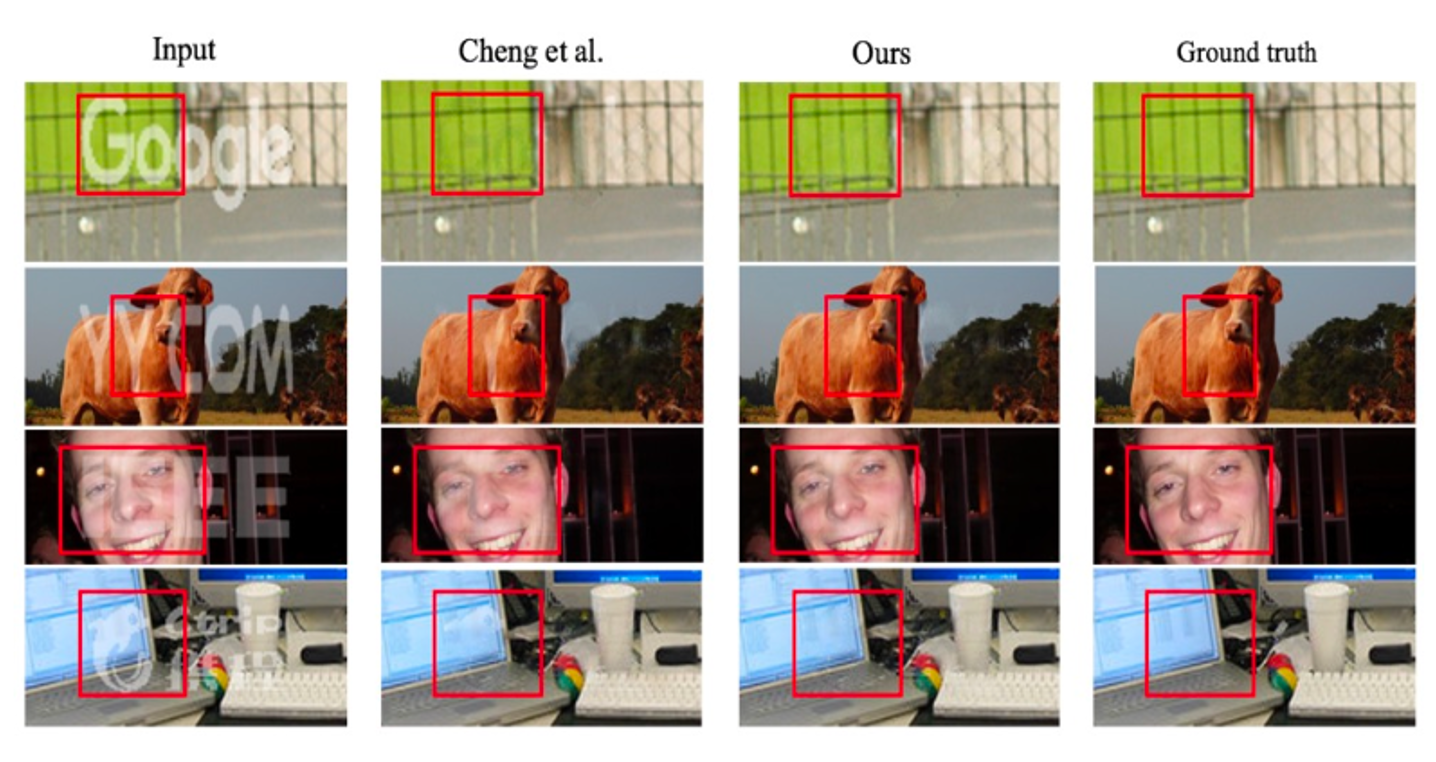
\includegraphics[width=\columnwidth]{21.png}
	\caption{水印去除结果}
	\label{fig:21}
\end{figure}

\subsection{两阶段水印去除架构}

\begin{figure}[!htbp]
	\centering
	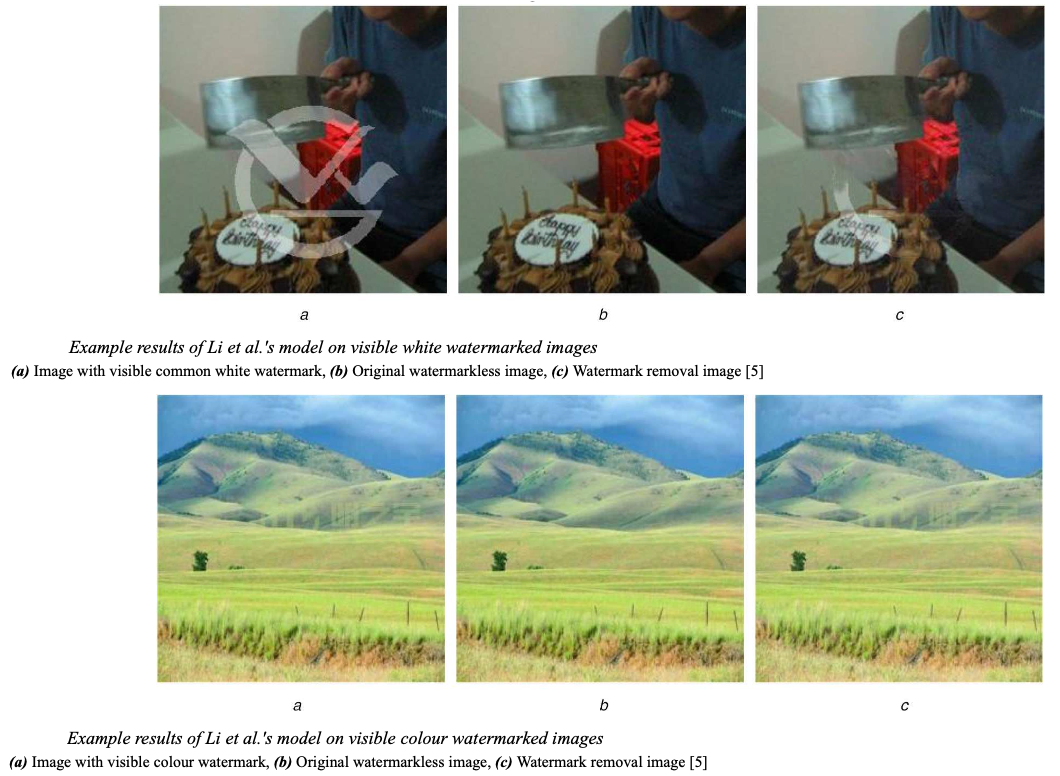
\includegraphics[width=\columnwidth]{22.png}
	\caption{研究动机}
	\label{fig:22}
\end{figure}

Li等在Cheng等定义的损失函数中引入了对抗性损失,使得生成的图像更加逼真。然而,对于白色水印图像,如图1所示,在去除水印后仍然存在残留水印。此外,Li等提出的方法无法去除颜色与背景颜色非常相似的可见水印,如图\ref{fig:22}所示。

基于上述观察,Jiang等~\cite{jiang2020two}提出了一种基于条件生成对抗网络(CGANs)和最小二乘生成对抗网络(least-squares generative adversarial networks, LSGANs)的可见水印去除网络架构。该架构包括水印提取和图像修复两个阶段。首先,第一阶段通过提取网络识别水印特征并提取图像中的水印,该网络主要关注水印图像的水印区域。然后,从水印图像中减去提取的水印,获得初步的去水印图像。最后,第二阶段将初步的去水印图像输入修复网络,以获得更一致和真实的去水印图像。

该工作延续了之前生成对抗网络和U-Net的模型设计,生成器包括提取网络和修复网络两个部分,同样使用两个判别器来区分生成的图像和真实图像。为了使提取的水印更接近真实水印,并使生成的无水印图像更接近真实图像,使用了两个有条件的PatchGAN判别器。与传统的判别器不同,它们可以判断图像中每个区域的真实概率。

\begin{figure*}[!htbp]
	\centering
	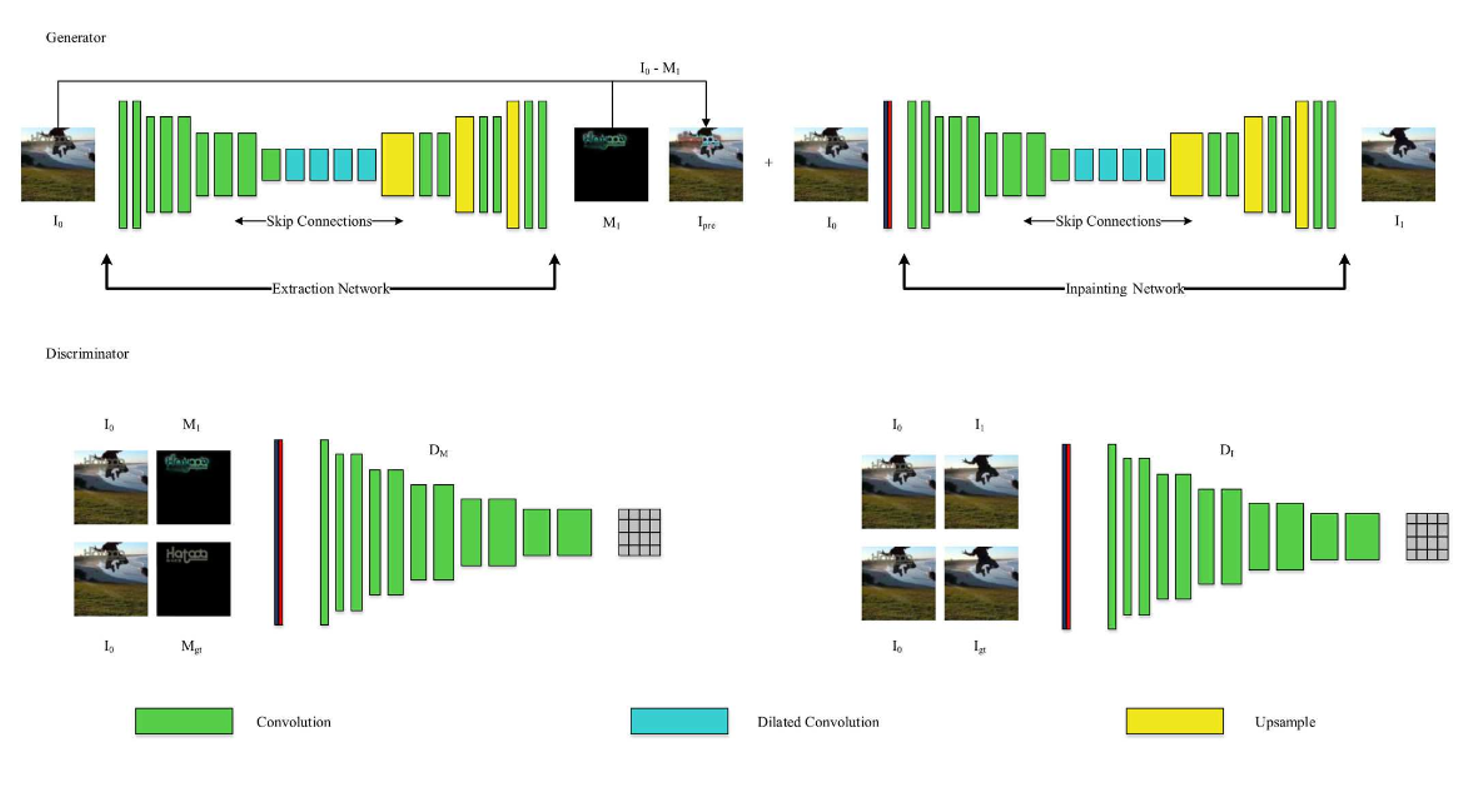
\includegraphics[width=\linewidth]{24.png}
	\caption{基于条件生成对抗网络和最小二乘生成对抗网络的两阶段水印去除框架示意图}
	\label{fig:24}
\end{figure*}


这是首个将图像修复与水印去除相结合的深度学习方法,网络整体更加关注于图像中水印的嵌入区域。该模型通过提取网络可以自动检测水印的位置,因而克服了传统水印去除方法需要手动标记水印区域的缺点。与基于深度学习的方法相比,Cheng等的方法依赖于现有的目标检测方法来检测水印位置,并且其去水印网络具有简单的结构和低效的损失函数。而本文的方法通过端到端训练可以直接为输入的水印图像输出无水印图像,并且由于增加了对抗性损失,输出的无水印图像更加逼真。此外,与Li等的工作相比,该模型更加关注水印区域,从而可以实现更鲁棒和逼真的水印去除。

\begin{figure}[!htbp]
	\centering
	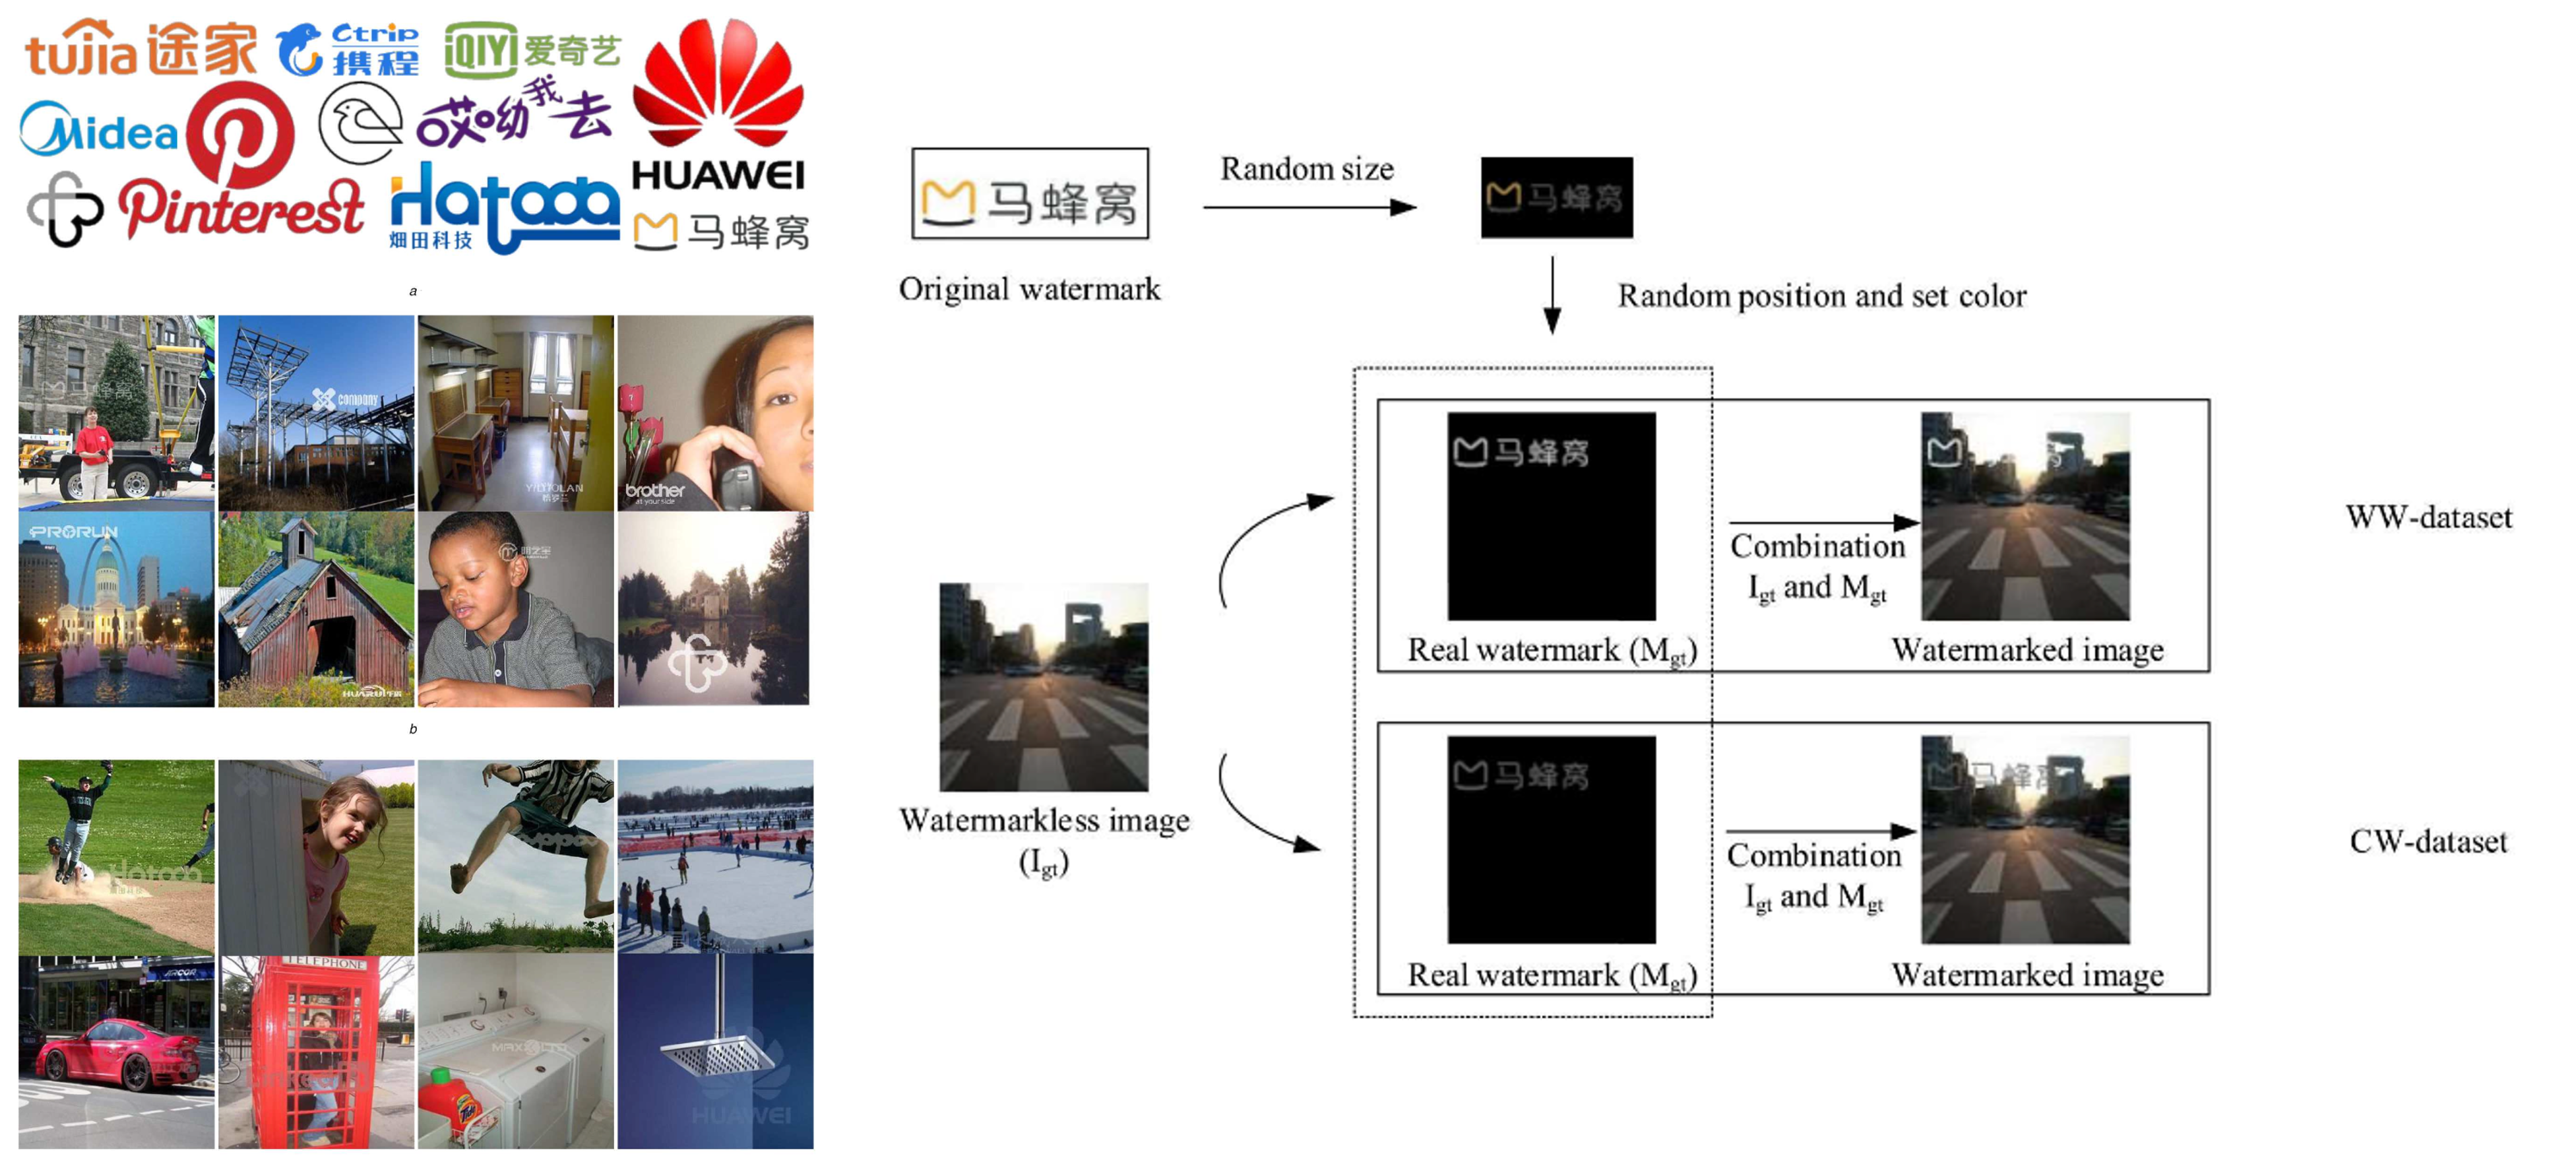
\includegraphics[width=\columnwidth]{23.png}
	\caption{WW数据集和CW数据集}
	\label{fig:23}
\end{figure}

为了评估网络架构的性能,Jiang等建立了两个带有水印的图像数据集——白色水印图像数据集(WW数据集)和彩色水印图像数据集(CW数据集)。两个数据集均包含53,300张带水印的图像,这些图像是由53,300张无水印的图像和100种原始水印生成的。其中53,300张无水印的图像来自于两个公共数据集,即PASCAL VOC2012和places2。而100种原始水印是从互联网上收集而来的品牌、网站等的标识。首先将53,300张无水印的图像平均分成100组(80组作为训练集,20组作为测试集)。然后,每个组中的图像都添加相同的水印,不同组的图像添加不同的水印。两个数据集之间唯一的区别是水印的颜色。如图\ref{fig:fig25}和\ref{fig:26}所示,实验结果表明,所提出的方法具有去除残留水印的能力,并且能够去除接近背景颜色的彩色水印。

\begin{figure}[!htbp]
	\centering
	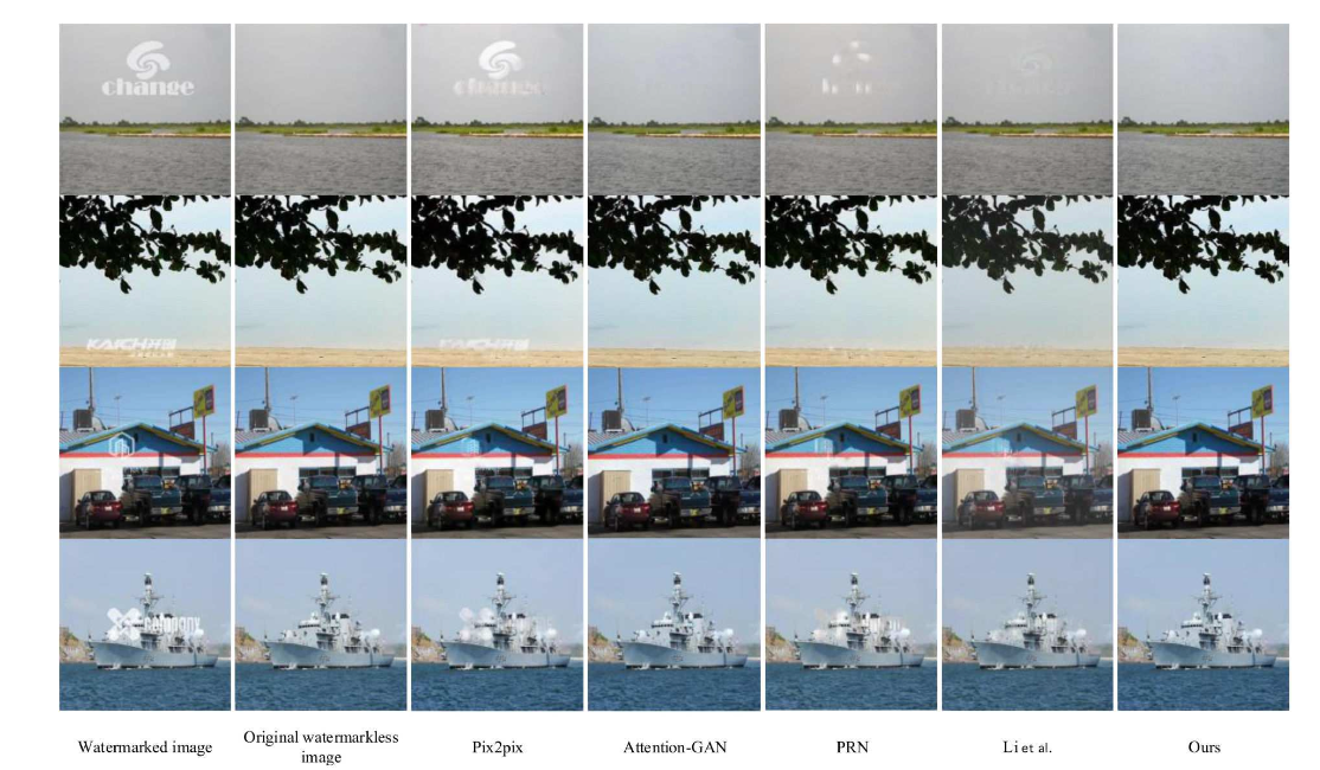
\includegraphics[width=\columnwidth]{25.png}
	\caption{WW数据集水印去除结果}
	\label{fig:25}
\end{figure}

\begin{figure}[!htbp]
	\centering
	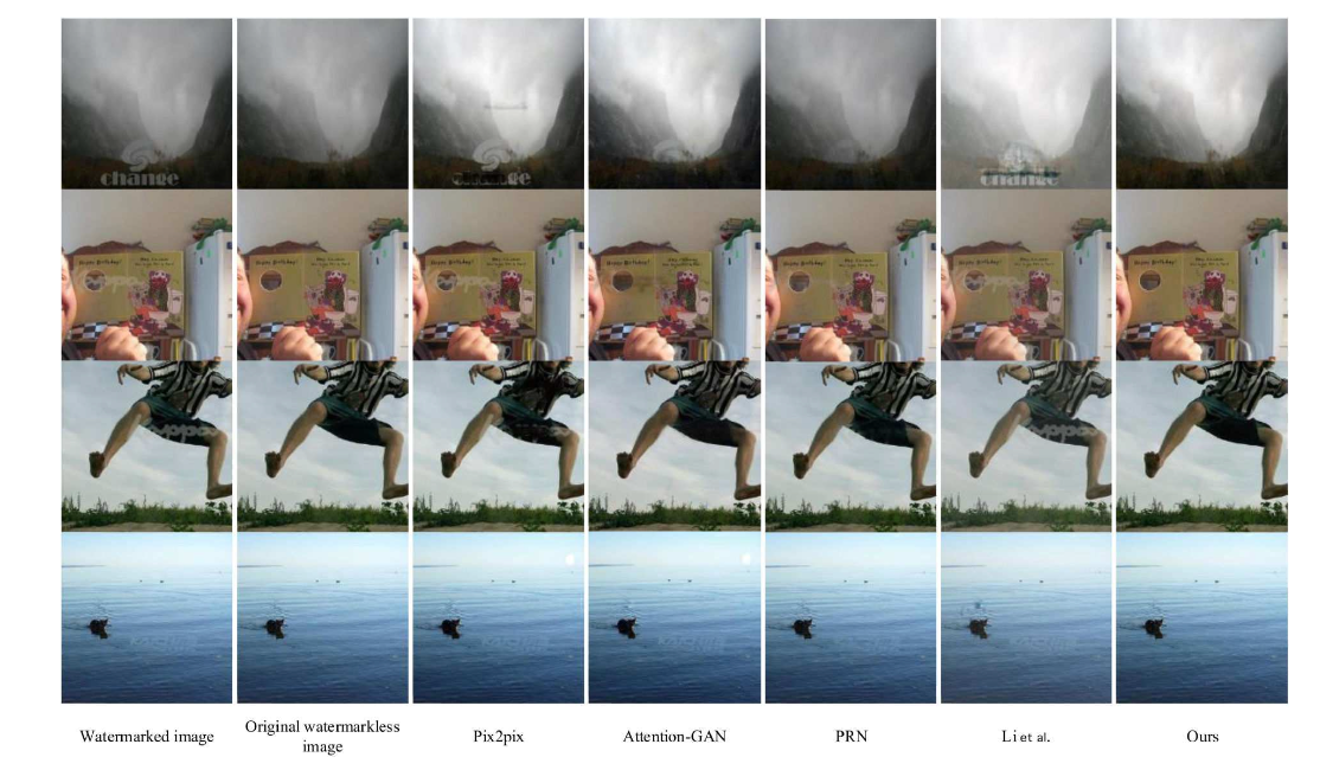
\includegraphics[width=\columnwidth]{26.png}
	\caption{CW数据集水印去除结果}
	\label{fig:26}
\end{figure}
